Es la distribución de todas las formas de radiación electromagnética, ordenadas según su longitud de onda y frecuencia. Incluye desde ondas de radio hasta rayos gamma. Para la medida de la longitud de onda se utiliza el nanómetro $(nm = m\text{x}10^{-9})$.

\begin{figure}[H]
  \centering
  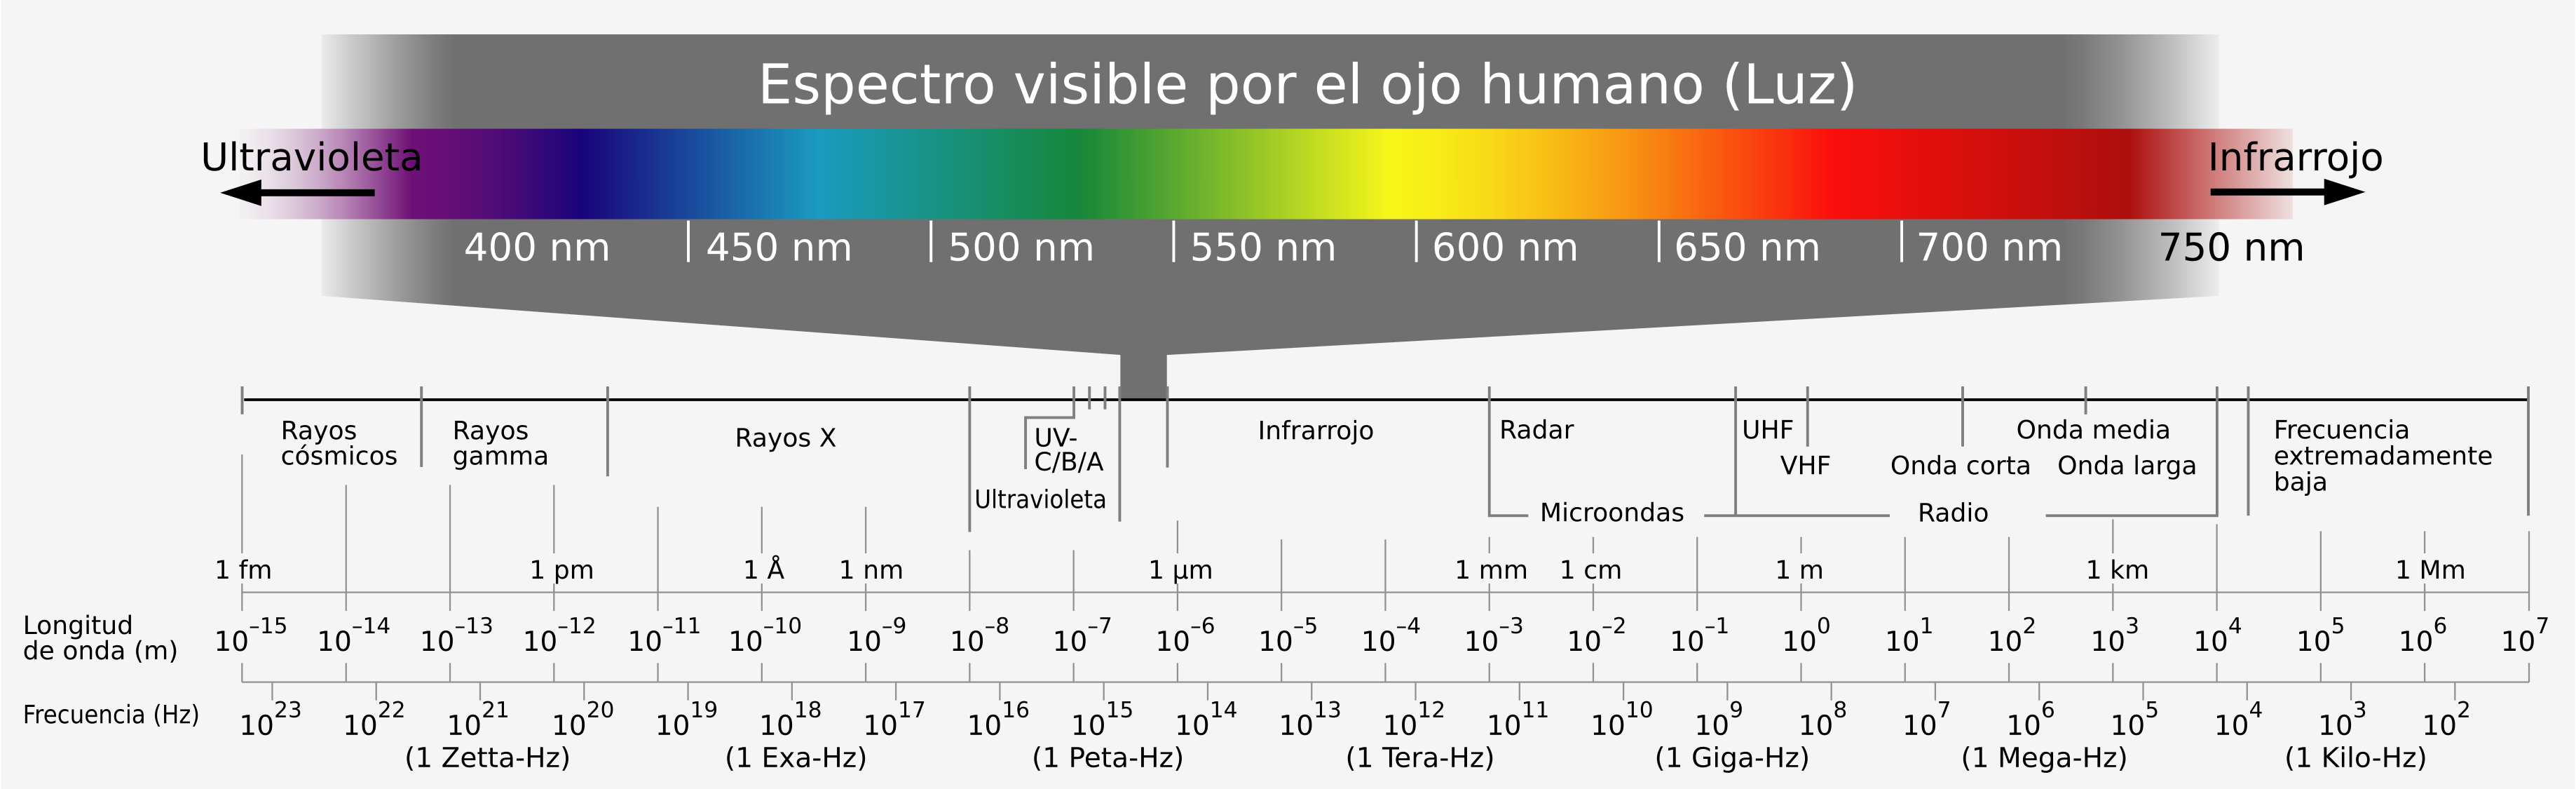
\includegraphics[scale=0.5]{imagenes/espectro_electromagnetico.png}
  \caption{Escpectro electromagnético\cite{wikielcmgnspc}}
\end{figure}

Las ondas cuya longitud de onda es alta viajan una mayor distancia, dado que pierden menos energía. Y aquellas donde es baja viajan menos distancia, pues pierden más energía. Esto se debe a la relación entre la frecuencia, longitud de onda y energía de una onda.

De mayor a menor longitud de onda se ordenan de la siguiente manera: ondas de radio, microondas, rayos infrarrojos, luz visible, rayos ultravioletas, rayos x y rayos gamma $(\gamma)$. Más allá se ubica la \textbf{radiación cósmica}.
